\documentclass[a4paper,11pt]{article}
\usepackage{fontspec}
\setmainfont{Times New Roman}
\usepackage{unicode-math}
\setmathfont{STIX Two Math}
\usepackage[margin=2.5cm]{geometry}
\usepackage{booktabs,graphicx,caption,setspace,ragged2e,tabularx,array}
\usepackage[authoryear,round]{natbib}
\usepackage{xurl}
\setstretch{1.3}
\setlength{\parindent}{0pt}
\setlength{\parskip}{6pt}
\setlength{\emergencystretch}{2em}
\renewcommand{\thesection}{S\arabic{section}}
\renewcommand{\thetable}{S\arabic{table}}
\renewcommand{\thefigure}{S\arabic{figure}}
\renewcommand{\theequation}{S\arabic{equation}}
\captionsetup{font=small,labelfont=bf,justification=raggedright,singlelinecheck=false}
\graphicspath{{../}}
\usepackage{longtable}
\usepackage{placeins}
% Keep floats within their owning section, subsection and subsubsection.
\let\OriginalSection\section
\renewcommand{\section}{\FloatBarrier\OriginalSection}
\let\OriginalSubsection\subsection
\renewcommand{\subsection}{\FloatBarrier\OriginalSubsection}
\let\OriginalSubsubsection\subsubsection
\renewcommand{\subsubsection}{\FloatBarrier\OriginalSubsubsection}

\begin{document}
\begin{center}
{\Large\bfseries Supplementary information}\par
\vspace{0.5em}
{\large Beyond thermal accumulation: improving cross-regional grapevine phenology prediction with terrain-aware forcing and residual learning}\par
\vspace{0.5em}
Linjia Yao, Qiang Yu and Gang Zhao
\end{center}

\section{Observation population and provenance}

The matched modelling population contains 74,618 accepted observations at 3,169
reported sites and 26,443 site--years during 1951--2025. Sites qualify through
any one of BBCH07, BBCH65, BBCH81 or BBCH89; complete stage sequences are not
required. The country distribution is unequal, and some country--stage
combinations contain no observations (Table~\ref{tab:country_population}).
Country-specific model comparisons therefore depend on stage-specific sample
sizes and attained predictions, rather than on the number of countries alone.
Record length ranges from one to 72 distinct years with at least one target
observation per site; gaps between years remain explicit and do not imply
continuous monitoring.

The seven original fields are the source-qualified site identifier, reported
variety, country, latitude, longitude, calendar date and directly recorded BBCH
code. Exact seven-field duplicates are removed, while different accepted dates
or cultivar labels remain separate. Empty variety labels are retained. A
record identifier is the SHA-256 digest of the seven-string JSON array, using
UTF-8 encoding, literal Unicode characters and compact comma/colon separators.
Source provenance retains every source occurrence, including exact duplicates,
and links excluded observations to the calendar or interval evidence used in
screening. Source-qualified site identifiers distinguish reporting systems;
they do not establish distinct physical vineyards, plants or cultivars.

The historical cleaned inventory contains 259,998 records across all stages. Its original weather-complete modelling cohort contains 74,311 target observations. The revised four-target inventory contains 75,738 records after direct-BBCH, source-quality, source-precedence and revised temporal screening. Matching to unchanged weather-eligible site--years, country and exact numeric coordinates yields 74,618 observations: 73,808 retained in common with the historical cohort, 810 restored and 503 historical records removed. The remaining 1,120 revised observations do not satisfy the unchanged matching requirements. Revised observations supply both final process calibration and residual learning. This weather-conditioned population does not represent a random sample of European vineyards.

\begin{table}[!htbp]
\centering
\caption{Frozen modelling population by country and BBCH stage. Sites are
source-qualified reported identifiers; site--years count distinct site and
calendar-year pairs. Zero denotes absence of eligible observations. Stage
columns contain observation counts, including accepted repeated observations.}
\label{tab:country_population}
\small
\resizebox{\textwidth}{!}{\begin{tabular}{lrrrrrrr}
\toprule
Country & Sites & Site--years & Records & 07 & 65 & 81 & 89 \\
\midrule
Bosnia and Herzegovina & 4 & 26 & 52 & 9 & 2 & 25 & 16 \\
Switzerland & 98 & 2,292 & 2,292 & 0 & 2,066 & 0 & 226 \\
Czechia & 3 & 56 & 94 & 0 & 47 & 47 & 0 \\
Germany & 1,375 & 16,253 & 55,732 & 21,221 & 21,008 & 13,503 & 0 \\
Spain & 5 & 47 & 83 & 18 & 14 & 30 & 21 \\
France & 1,620 & 6,740 & 13,897 & 2,628 & 2,802 & 4,370 & 4,097 \\
Croatia & 5 & 251 & 940 & 471 & 0 & 464 & 5 \\
Luxembourg & 1 & 37 & 72 & 37 & 0 & 35 & 0 \\
Montenegro & 2 & 5 & 18 & 9 & 0 & 3 & 6 \\
Sweden & 1 & 1 & 1 & 0 & 1 & 0 & 0 \\
Slovakia & 55 & 735 & 1,437 & 723 & 714 & 0 & 0 \\
\midrule
Total & 3,169 & 26,443 & 74,618 & 25,116 & 26,654 & 18,477 & 4,371 \\
\bottomrule
\end{tabular}
}
\end{table}

\section{Meteorological and terrain matching}

All retained site--years have finite daily mean temperatures from 4 June of
the preceding year through 31 December of the observation year. This window
covers the preceding-September chilling origin and the 90-day histories used
by residual models. Eligibility concerns actual daily values and dates, not
the existence of an extraction request or file. No missing temperature is
interpolated, and nearby coordinates do not authorize reuse. RAW temperatures
and recalculated DEM temperatures are stored in an independent publication
snapshot; prior weather exports retain their original provenance.

The underlying ERA5-Land reanalysis is documented by
\citet{munozSabaterERA5Land2021}. The extraction workflow uses the Earth Engine
collection \texttt{ECMWF/ERA5\_LAND/DAILY\_AGGR} for daily forcing and
\texttt{ECMWF/ERA5\_LAND/MONTHLY\_AGGR} for climate profiles. Their parent hourly
and monthly data products have separate dataset identifiers
\citep{copernicusClimateChangeServiceERA5LandHourly2019,copernicusClimateChangeServiceERA5LandMonthly2019}.
Reused samples retain their recorded extraction provenance.

Native ERA5-Land sampling uses the regular 0.1$^{\circ}$ grid. The sampling
transform has a longitude origin of $-180.05^{\circ}$ and a latitude origin
of $90.05^{\circ}$, with steps of $0.1^{\circ}$ and $-0.1^{\circ}$,
respectively. Actual pixel identities resolve points on cell boundaries.
The matched sites occupy 1,792 sampled cells. Grid elevation is the official
ERA5-Land invariant geopotential divided by 9.80665~m~s$^{-2}$; it is not the
mean Copernicus elevation of a weather-grid cell. The temperature correction is
$T_{\mathrm{DEM}}=T_{\mathrm{RAW}}-0.0065(z_{\mathrm{site}}-z_{\mathrm{grid}})$,
with elevations in metres and temperature in degrees Celsius. It modifies
gridded forcing and does not create an independent local temperature measurement.

Copernicus GLO-30 supplies site elevation from the containing native raster
pixel \citep{esaAirbusCopernicusDEM2022}. Slope and aspect use a 3$\times$3 neighbourhood, and local elevation
variability is the population standard deviation over finite pixels in an
11$\times$11 neighbourhood. Actual raster transforms and extents determine
tile containment, including coordinates on geographic degree boundaries.
Source-pixel values, finite-pixel counts and hashes identify the sampled
neighbourhoods. Incomplete edge neighbourhoods retain explicit missing
derivatives or reduced variability support; pixel values are not invented.
Missing terrain predictors are imputed within residual-model training folds.
The DEM represents surface elevation, so vegetation, structures, coordinate
uncertainty and spatial resolution can affect interpretation of local metrics.

\section{Validation populations and weighting}

Conservative independence groups connect sites that share an actual weather
cell, exact coordinates or coordinates rounded to four decimal places. This
transitive grouping restricts validation leakage without asserting individual
vineyard identity. The primary design allocates complete groups within five
environmental zones to calibration or test sets. Monthly temperature profiles
cover 1991--2020 and use RAW forcing; standardization and clustering operate
on unique weather cells rather than weighting frequently reported cells more
heavily. Country labels, event dates and model errors do not determine zones.

Table~\ref{tab:protocol_population} gives the active primary site-holdout population after revised screening. Calibration contains 59,472 observations from 2,534 reported sites and 1,434 independence groups; testing contains 15,146 observations from 635 sites and 357 groups. The original allocation used 1,792 unique weather cells, while the revised observed population retains 1,791 weather cells and 1,791 independence groups. Temperature-zone centroids and site assignments remain those defined before revised screening. Four complete calibration-group folds support ordinary and nested cross-fitting. Historical spatial, warm-year, warm-site and unstratified protocols are not final-performance evaluations of the median-cutoff or TabM models.

\begin{table}[!htbp]
\centering
\caption{Active primary calibration and test populations after revised screening. The last four columns contain observations of BBCH07, BBCH65, BBCH81 and BBCH89. Groups are the unchanged conservative independence units; no group spans calibration and testing.}

\label{tab:protocol_population}
\small
\resizebox{\textwidth}{!}{\begin{tabular}{llrrrrrr}
\toprule
Protocol & Partition & Sites & Groups & 07 & 65 & 81 & 89 \\
\midrule
Environmental-zone sites & Calibration & 2,534 & 1,434 & 20,043 & 21,185 & 14,723 & 3,521 \\
Environmental-zone sites & Test & 635 & 357 & 5,073 & 5,469 & 3,754 & 850 \\
\bottomrule
\end{tabular}
}
\end{table}

Prediction errors are signed calendar-day differences, predicted minus
observed. For each stage, squared or absolute errors are averaged within each
reported site and then equally across sites; RMSE takes the square root after
this equal-site mean squared error. Early calibration averages the three BBCH07/65/81 site-balanced MAEs under
separate bias and raw-attainment constraints; maturity uses a weighted median requirement. Different accepted observations sharing a site--year--stage
receive the same model prediction and retain separate within-site error
contributions. Neither the total number of observations nor the number of
sites is a substitute for the number of independent validation groups.

Paired RAW/DEM and process/residual comparisons preserve common observed records. The final paired effects compare scoring errors for RAW versus DEM process-based models, RAW versus DEM hybrids, and process versus hybrid predictions under each temperature input. Scoring-date contrasts apply the fixed administrative dates for BBCH81 and BBCH89 without treating those dates as attained events; raw-date performance is summarized separately on attained predictions. Raw attainment, by-cutoff attainment and administrative assignment retain their full observation denominators. Independent-group bootstrap resampling preserves all sites within each selected group and equal-site weighting; intervals use 2,000 replicates, require at least ten contributing original groups in each reported stage and retain percentile limits only when at least 95\% of resamples are finite. Overall effects weight all four stages equally and require the ten-group minimum in every stage. Calibration intervals describe apparent fitted-model comparisons; test intervals concern held-out sites. Terrain correlations and slopes describe predictive associations, without causal interpretation.

\section{Fixed responses and calibrated requirements}

Ten process structures share fixed temperature-response components. Linear
forcing has a 0~$^{\circ}$C base; the beta forcing cardinals are 0, 25.4 and
35~$^{\circ}$C. Triangular and beta chilling share cardinals of $-1.7$, 1.7
and 13.2~$^{\circ}$C. These controls follow the documented GFV base and Fila
parameterizations, with their transfer to four stages and alternative response
families treated as adaptations \citep{parkerGeneralPhenologicalModel2011a,filaComparisonDifferentModelling2014}.
Forcing-only models start on 1 January; chilling starts on 1 September of the
preceding year. Parallel minimum forcing competence is fixed at 0.2 as a
project choice. These fixed quantities are not newly estimated physiological
constants for the European observation domain.

\begin{table}[!htbp]
\centering
\caption{Adjustable parameter counts and inclusive numerical search ranges.
Every structure has four stage-specific forcing requirements; chilling models
add one common chilling requirement. Linear forcing accumulates degree-days
above 0~$^{\circ}$C; beta forcing and both chilling responses accumulate daily
response units. Ranges apply separately to each forcing requirement and do
not represent physiological limits.}
\label{tab:parameter_bounds}
\small
\begin{tabular}{llrll}
\toprule
Structure & Interaction & Fitted & Forcing range & Chilling range \\
\midrule
FL & none & 4 & 0.001--3000 & --- \\
FB & none & 4 & 0.001--200 & --- \\
CL-FL-S & sequential & 5 & 0.001--3000 & 0.001--200 \\
CL-FL-P & parallel & 5 & 0.001--3000 & 0.001--200 \\
CB-FL-S & sequential & 5 & 0.001--3000 & 0.001--200 \\
CB-FL-P & parallel & 5 & 0.001--3000 & 0.001--200 \\
CL-FB-S & sequential & 5 & 0.001--200 & 0.001--200 \\
CL-FB-P & parallel & 5 & 0.001--200 & 0.001--200 \\
CB-FB-S & sequential & 5 & 0.001--200 & 0.001--200 \\
CB-FB-P & parallel & 5 & 0.001--200 & 0.001--200 \\
\bottomrule
\end{tabular}

\end{table}

Requirements are shared across sites, years and reported varieties within each process structure and temperature input, with parameter counts and search ranges given in Table~\ref{tab:parameter_bounds}. The three early forcing requirements and any chilling requirement are fitted jointly; the maturity requirement is subsequently set to the equal-site weighted median of valid positive thermal requirements from the day after raw predicted BBCH81 to observed BBCH89. Early parameters and raw predictions remain unchanged by this median step. After each attained stage, forcing resets and accumulation for the next stage begins on the following day; overshoot is discarded. Observed dates never initialize simulation. Sequential budburst requires chilling completion, whereas parallel budburst can precede full chilling competence.

The optimizer targets absolute site-balanced bias of at most one day and raw attainment of at least 99\% at both record and equal-site levels for BBCH07, BBCH65 and BBCH81. It first seeks bias feasibility and then reduces mean early-stage site-balanced MAE when feasible. The latest calibration maturity month--day, 4 November, is fixed across all folds for BBCH81/89 administrative scoring. Maturity has no full-attainment constraint. Three seeds, 20260907--20260909, use 300-generation initial searches and a 600-generation retry limit, with population multiplier fifteen, relative tolerance 0.001 and no polishing. Unmet targets and convergence remain explicit diagnostics. Supplementary Methods S7 gives the objective and median definition; compiled numerical acceleration preserves the canonical raw simulation dates.

\section{Historical screening sensitivity and hybrid order constraints}

The historical observation-screening sensitivity restored quarantined records only when
their original country, exact coordinates and site--year match the frozen
modelling population. It added 1,598 records to the historical 74,311 accepted observations
(Table~\ref{tab:screening_population}). These records are ambiguous evidence,
not verified physiological extremes or established ground truth. Of the
11,034 quarantined inventory records, 8,954 concern non-target stages and 482
target records occur outside the frozen site--year population. Neither class
enters this sensitivity population.

\begin{table}[!htbp]
\centering
\caption{Historical screening-sensitivity population within unchanged frozen sites and
years, preceding the active revised calibration. Restored records retain their original dates, BBCH codes and identities.
Calibration/test labels are inherited from the primary environmental-zone split;
restoration changes the evaluation population and does not refit either
process or residual models.}
\label{tab:screening_population}
\small
\begin{tabular}{lrrrr}
\toprule
Stage & Retained & Restored & Calibration restored & Test restored \\
\midrule
BBCH07 & 24,934 & 338 & 266 & 72 \\
BBCH65 & 26,427 & 766 & 609 & 157 \\
BBCH81 & 18,644 & 403 & 329 & 74 \\
BBCH89 & 4,306 & 91 & 80 & 11 \\
\bottomrule
\end{tabular}

\end{table}

This historical accepted-versus-augmented comparison reused earlier locked process and residual models. It is distinct from the active 74,618-record revised population and does not establish the sensitivity of the final median-cutoff and TabM results. The final calibration uses revised observations under the source-quality and four-target rules in Supplementary Methods S6. Counts by screening rule overlap when a record has multiple exclusion reasons. Historical date and interval thresholds never constrain raw predictions.

Hybrid dates include an integer-day residual correction, rounded to the
nearest even integer at half-day ties. A subsequent ordering step requires
each attained corrected stage to occur at least one day after the preceding
attained corrected stage. Unconstrained corrected dates and the additional
days introduced by ordering are retained separately. Their paired error
comparison isolates the ordering step; it does not estimate the effect of
rounding or the full residual learner. Adjustment frequencies distinguish
site--year--stage predictions represented by observed records from the number
of repeated observation rows. Missing predictions remain missing under both
date representations.

\section{Seasonal and chronological observation screening}
Seasonal timing and the order and duration of developmental phases were checked after duplicate removal. The screening thresholds were defined for this European dataset; they are not universal physiological limits and were not derived from model residuals. Observed dates and stage codes were not corrected, and the thresholds are not imposed on model predictions.

Calendar screening required a valid observed date within the inclusive window for its recorded stage. The original target-stage windows were 1 February--15 June for BBCH07, 1 May--31 July for BBCH65, 1 July--15 October for BBCH81 and 15 July--15 November for BBCH89. Main Table~2 gives the active revised windows. A date exactly on either boundary remained eligible; a date outside either boundary was quarantined with its original fields, stage code, date and failed-window evidence. Dates were compared by month and day so that leap years were treated consistently. No date was moved to a boundary, repaired or inferred from another stage. Passing a calendar window did not establish observation validity or exempt a record from subsequent chronology checks.

Non-target stages retained their original screening windows: BBCH01--09, 1 February--15 June; BBCH10--19, 1 March--31 July; BBCH50--59, 1 April--15 July; BBCH60--69, 1 May--31 July; BBCH70--79, 15 May--15 September; BBCH80--85, 1 July--15 October; and BBCH86--89, 15 July--15 November. These stages contributed chronology evidence to the historical full-inventory screen but do not constrain the active four-target reassessment. No seasonal window was imposed on BBCH00, BBCH90--99 or unlisted stage families. Dormancy and late-season development can extend across calendar years.

An observation qualified for the four-stage target export when its recorded code was one of BBCH07, 65, 81 or 89 and it survived the inventory checks. Missing observations at the other target stages did not exclude a site or season. Subsequent weather and independence requirements defined modelling eligibility separately from calendar eligibility.



Stage order and phase duration were assessed within each site, reported variety and calendar year. Observations without a variety name were grouped separately from named cultivars. These groups, and those defined by DWD maturity classes, may include several plants or cultivars, so inconsistent dates cannot necessarily be attributed to an error in an individual plant.

Two developmental sequences were assessed separately: bud and leaf development (BBCH01, 03, 05, 07, 09 and 10--19) and reproductive development (BBCH01, 03, 05, 07, 09, 53, 55, 57, 60--69, 71, 73, 75, 77, 79, 81, 83, 85, 87 and 89). All observed stage pairs within each sequence were compared. Separate sequences allowed leaf and reproductive development to overlap without imposing an order based solely on their numerical BBCH codes. BBCH00 and BBCH90--99 were excluded from these comparisons.

A later stage could occur on the same date as an earlier stage, but not before it. The historical adjacent bounds were 20--100 days for BBCH07 or BBCH09 to BBCH65, 30--120 days for BBCH65 to BBCH81 and 10--90 days for BBCH81 to BBCH89. Main Table~3 gives the six bounds for the active four-target screen. BBCH07 and BBCH09 were treated as distinct budburst observations. The interval rules applied only to the listed stages; missing stages were neither inferred nor grounds for exclusion.



Interval checks were applied to observations that passed the seasonal screen. For each pair of observed stages, every date required at least one date at the other stage that satisfied the interval criterion. A date that failed this check was excluded even if another observation of the same stage was compatible. When no compatible pair existed, observations of both stages were excluded because the erroneous date could not be identified. All exclusions were determined from the same set of observations and applied simultaneously in each iteration. Checks were repeated until no further exclusions occurred. Stages with no remaining observations imposed no additional constraint, and unrelated stages were retained. Screening excluded 11,034 observations (4.1\%), leaving 259,998 observations. Excluded records remain available for sensitivity analysis because unusual weather, reporting intervals and management practices may also produce atypical dates.



\subsection*{Revised four-target screening for the active calibration and test population}
The revised cohort is reconstructed from the same verified original source tables, retaining direct BBCH07, 65, 81 and 89 observations from 1951 onward after exact seven-field deduplication. It supersedes the historical observation selection for final calibration and testing while preserving the original weather eligibility and site assignments. Source quality and report reconciliation precede the revised calendar windows in Main Table~2. The revised flowering and veraison windows begin on 1 April and 1 June, respectively. These earlier boundaries broaden the range of eligible dates and are project screening choices, not physiological limits or cutoffs estimated from model residuals. They do not independently validate individual records; compatible stage intervals and source-quality requirements remain necessary for retention.

Within each source-qualified site, exact reported variety label and year, adjacent target intervals are 20--120 days for 07$\to$65, 30--120 days for 65$\to$81 and 10--90 days for 81$\to$89. The 120-day upper bound for 07$\to$65 retains room for early budburst; the original inventory includes two February-to-flowering pairs spanning 108 days. These pairs are descriptive evidence, not independently verified reference events. Summing adjacent bounds gives 50--240 days for 07$\to$81, 40--210 days for 65$\to$89 and 60--330 days for 07$\to$89. Cross-stage bounds remain testable when intermediate stages are missing; no missing date is imputed. Each record requires a compatible date at every other observed target stage. Unsupported records are removed simultaneously and checked until stable. Unlike the original full-inventory screen, non-target stages do not constrain this four-target reassessment. Restored observations can therefore reflect the changed comparison scope as well as revised calendar or interval bounds.

DWD quality is evaluated at the highest available control level for each exact observation. Flags for incorrect or doubtful dates exclude the record unless a no-objection, corrected or confirmed flag resolves doubt at that same level; an incorrect flag takes precedence. Corrected and confirmed dates remain eligible. Where the station, maturity-class label, year, BBCH, original object identifier and original phase identifier agree, one quality-controlled annual date takes precedence over conflicting immediate reports below quality level 7. This is a declared source-precedence policy, not proof that every immediate report represents a revision of the same biological observation. Equally controlled alternatives and records without quality metadata are not resolved by an arbitrary minimum or median. Empty variety labels remain separate from named varieties, and repeated accepted dates retain ambiguity flags. The quality-level and date-flag meanings follow the DWD annual grapevine data documentation.

The revised inventory contains 75,738 retained target observations and 1,575 quarantined observations. Relative to the original phenology-only target inventory, 503 previously retained records are excluded and 1,008 previously quarantined records are restored. Original seven fields, source occurrences, event hashes and exclusion evidence remain recoverable. Weather and identity matching retain 74,618 observations, including 810 restored observations, in unchanged eligible site--years. Final process and neural calibration use 59,472 of these observations; the 15,146 held-out observations preserve their original site assignments. The screen was revised after preliminary model results became available, although its rules do not use residuals. Consequently, differences from historical results combine changes in eligibility and calibration and are not an unbiased estimate of a cleaning benefit.

\section{Detailed process equations and numerical conventions}

Six function combinations pair two forcing functions with three chilling options (the main model catalogue). The two forcing-only combinations and sequential and parallel variants of the four chilling--forcing combinations give ten process-based model structures. Linear forcing (FL) accumulates thermal time above a fixed base temperature. Beta forcing (FB) represents a nonlinear response that peaks at an optimum temperature and declines to zero at the upper temperature limit. Beta forcing and beta chilling (CB) follow the response families examined by \citet{filaComparisonDifferentModelling2014}. Piecewise-linear chilling (CL) uses the triangular response described by \citet{deWergifosseHETEROFOR2020}, following H\"anninen (1990). This chilling function was developed for forest trees; its application to grapevine is an adaptation. Temperature-response parameters are fixed from literature and shared across stages, sites and models wherever the same component occurs; only accumulation requirements are calibrated.

\paragraph{Daily temperature responses.}
All process-based models use daily mean air temperature $T_t$ in $^{\circ}$C. For target stage $s\in\mathcal{S}=\{07,65,81,89\}$, linear forcing is

\begin{equation}
R^{\mathrm{FL}}_{f,s}(T_t)=\max(T_t-T_b,0),
\label{eq:linear_forcing}
\end{equation}

where $T_b=0$~$^{\circ}$C for all stages, following the base temperature of the GFV model \citep{parkerGeneralPhenologicalModel2011a}. GFV originally targets flowering and veraison; use of this base for the complete four-stage sequence is an extension, not an exact reproduction of GFV. Summation over daily time steps gives thermal time in $^{\circ}$C\,d. The normalized beta response is

\begin{equation}
B(T;a,b,c)=
\begin{cases}
\displaystyle\frac{c-T}{c-b}
\left(\frac{T-a}{b-a}\right)^{\!\frac{b-a}{c-b}}, & a<T<c,\\[6pt]
0, & T\leq a\ \text{or}\ T\geq c,
\end{cases}
\label{eq:beta_response}
\end{equation}

where $a<b<c$ are the minimum, optimum and maximum temperatures, respectively, and $B(b;a,b,c)=1$ \citep{filaComparisonDifferentModelling2014}. Beta forcing uses $R^{\mathrm{FB}}_{f,s}(T_t)=B(T_t;0,25.4,35)$ for every stage. The optimum of 25.4~$^{\circ}$C is the shared forcing optimum of Fila et al.'s Fbeta5* model (Table~8), calibrated using field and growth-room observations; the lower and upper limits of 0 and 35~$^{\circ}$C follow their adopted beta formulation. Beta chilling uses $R^{\mathrm{CB}}_c(T_t)=B(T_t;T_{c,\min},T_{c,\mathrm{opt}},T_{c,\max})$. Its fixed cardinal temperatures are $-1.7$, 1.7 and 13.2~$^{\circ}$C, respectively, from the CF10* parameterization informed by field and growth-room observations in their Table~7. The alternative CL response is

\begin{equation}
R^{\mathrm{CL}}_c(T)=
\begin{cases}
0, & T\leq T_{c,\min}\ \text{or}\ T\geq T_{c,\max},\\[3pt]
\dfrac{T-T_{c,\min}}{T_{c,\mathrm{opt}}-T_{c,\min}}, & T_{c,\min}<T\leq T_{c,\mathrm{opt}},\\[6pt]
\dfrac{T_{c,\max}-T}{T_{c,\max}-T_{c,\mathrm{opt}}}, & T_{c,\mathrm{opt}}<T<T_{c,\max}.
\end{cases}
\label{eq:triangular_chilling}
\end{equation}

CL uses the same three chilling temperatures as CB, so the contrast changes curve shape without changing its temperature limits or optimum (main Fig.~3). These cardinals originate from grapevine beta chilling, not from the forest-tree parameterization of the triangular function. Both chilling responses are bounded between zero and one. Their cumulative sums, and those of beta forcing, are expressed as accumulated daily response units; they are not interchangeable with the degree-day sums of linear forcing.

\paragraph{Accumulation and stage progression.}
Each site--year is simulated independently through 31 December of the observation year. Forcing-only models start on 1 January ($t_0=1$), a common calendar convention discussed by \citet{filaComparisonDifferentModelling2014}. This date is fixed across sites, years and forcing functions, and differs from the day-60 origin of the original GFV model. The first day contributes to accumulation. Calendar start dates are not calibrated in the structure comparison.

For a stage starting on date $\tau_s$, cumulative effective forcing and its predicted occurrence date are

\begin{equation}
F_s(t)=\sum_{u=\tau_s}^{t}w_{s,u}R_{f,s}(T_u),\qquad
\widehat{D}_s=\min\{t\geq\tau_s:F_s(t)\geq H_s\},
\label{eq:stage_accumulation}
\end{equation}

where $H_s>0$ is the stage-specific forcing requirement and $w_{s,u}=1$ except during budburst forcing in parallel models. After each predicted stage, the forcing sum is reset to zero and accumulation for the next stage begins on the following day: $\tau_{65}=\widehat{D}_{07}+1$, $\tau_{81}=\widehat{D}_{65}+1$ and $\tau_{89}=\widehat{D}_{81}+1$. Threshold overshoot is discarded, and no day's forcing contributes to two stages. The four requirements therefore describe successive developmental intervals, not cumulative thresholds from a common starting date. Observed preceding-stage dates never initialize predictions, including during calibration or when intermediate observations are missing.

\paragraph{Chilling--forcing interaction.}
Chilling accumulates from $t_c$, 1 September of the preceding year, with zero initial chilling:

\begin{equation}
C(t)=\sum_{u=t_c}^{t}R_c(T_u),\qquad
t_C=\min\{t\geq t_c:C(t)\geq C_{\mathrm{crit}}\},
\label{eq:chilling_accumulation}
\end{equation}

where $C_{\mathrm{crit}}>0$ is the fitted chilling requirement. In sequential models, budburst forcing begins on $\tau_{07}=t_C+1$; forcing before chilling completion is excluded. In parallel models, chilling and budburst forcing both start on $t_c$, allowing the two processes to overlap \citep{chuineUnifiedModelBudburst2000}. Daily budburst forcing is multiplied by a competence factor adapted from \citet{liuSimulatingOnsetSpring2018}:
\begin{equation}
K_t = K_{\min} + (1-K_{\min})\min\!\left(\frac{C(t-1)}{C_{\mathrm{crit}}},1\right),
\label{eq:parallel_competence}
\end{equation}

with $w_{07,t}=K_t$ in Eq.~\ref{eq:stage_accumulation}. Here $C(t-1)$ is chilling accumulated before the current day and $C(t_c-1)=0$. The minimum competence is fixed at $K_{\min}=0.2$ across parallel models as an experimental control, not as a literature-established grapevine constant. Full chilling marks full forcing competence, not an additional condition for budburst; parallel models can therefore predict budburst before $C_{\mathrm{crit}}$ is reached. Chilling does not modify forcing after budburst, and the stage sequence remains identical under sequential and parallel interactions.

\paragraph{Parameter sharing and search bounds.}
The early forcing requirements $H_{07}$, $H_{65}$ and $H_{81}$ are calibrated jointly, together with any chilling requirement; $H_{89}$ is estimated subsequently by the weighted-median procedure. Each requirement is shared across sites, years and cultivars, rather than estimated separately for individual locations. Chilling models additionally calibrate one $C_{\mathrm{crit}}$ for dormancy release, also shared across sites and years. Thresholds can differ among model structures and temperature treatments, but temperature-response parameters remain identical wherever the corresponding component is present. Repeated accepted observations at the same site--year--stage are compared with the same simulated date and remain separate contributions to the fitting loss.

Linear forcing requirements are searched between 0.001 and 3000~$^{\circ}$C\,d; beta forcing and chilling requirements are searched between 0.001 and 200 daily response units. The larger allowance for linear forcing accommodates accumulation above a fixed 0~$^{\circ}$C base. These are numerical search limits, not physiological bounds. Parameter-boundary proximity is recorded; the fitting pipeline does not enlarge bounds automatically. Forcing-only models therefore have four fitted parameters, and both sequential and parallel chilling--forcing models have five. No temperature-response, calendar-start or competence parameters are fitted in this comparison.

The fixed temperatures provide literature-based controls for comparing model structures, not universal physiological constants. The Fila parameter sets were estimated for Chardonnay in northeastern Italy, whereas the observation collection spans multiple cultivars and climates. In particular, chilling effectiveness above 10~$^{\circ}$C remained uncertain in that study, and transfer of its cardinals to triangular chilling and of its forcing response to BBCH89 requires independent evaluation. Structural comparisons are therefore conditional on the selected response parameters. The factorial experiment does not vary these cardinals, calendar origins or minimum competence, so it does not establish robustness to alternative fixed settings.



\paragraph{Early-stage calibration and numerical safeguards.}
For each stage $s\in\{07,65,81\}$, scored errors are averaged first within each site and then equally across sites. Their mean absolute value is $A_s$ and their signed mean is $B_s$. BBCH07 and BBCH65 use attained raw dates; BBCH81 uses its raw date if attained on or before 4 November and the administrative cutoff otherwise. Sites without a scored date do not enter the finite-date error average, but their missing predictions remain in raw-attainment denominators. Repeated accepted records retain separate contributions within a site--stage.
\begin{equation}
L_{\mathrm{early}}=\frac{1}{3}\sum_{s\in\{07,65,81\}} A_s,
\qquad V=\max\left(0,\max_{s\in\{07,65,81\}}|B_s|-1\right).
\label{eq:calibration_loss}
\end{equation}
The first optimization minimizes $V$ subject to record-level and equal-site raw attainment of at least 0.99 for every early stage. If $V=0$ is achieved, a second optimization minimizes $L_{\mathrm{early}}$ while retaining both bias and coverage constraints. Otherwise the smallest attained $V$, with MAE as tie-breaker, determines the coverage-admissible candidate, and the unmet bias target is recorded. BBCH89 never contributes to these objectives. Administrative BBCH81 assignment cannot satisfy or conceal a failure of its raw-attainment constraint.

Differential evolution uses seeds 20260907, 20260908 and 20260909, population multiplier 15, 300 initial generations, relative tolerance 0.001, one evaluation worker and no polishing. Retry searches permit 600 generations with the same seeds and bounds. Bias feasibility can end before a retry if a feasible candidate already exists; unsuccessful convergence otherwise permits the extended budget. A finite best candidate may remain unconverged, and convergence does not by itself imply that the bias target was attained. Full-calibration early fitting can initialize from an earlier calibration-only process fit. Ordinary and nested cross-fitting instead initialize from fixed response parameters and predeclared thresholds of $0.001+10^{-9}$; the numerical offset prevents lower-bound rounding in the optimizer and contains no label information. Parameters fitted using excluded folds never initialize those refits. Failure of this predeclared start to attain the raw-coverage floor is recorded without a full-fit fallback.

\paragraph{Median maturity requirement.}
With early parameters fixed, a calibration maturity observation at site $j$ supplies
\begin{equation}
Q_{ji}=\sum_{t=\widehat D_{81,ji}+1}^{D_{89,ji}}R_{f,89}(T_t),
\qquad w_{ji}=\frac{1}{n_j^{\mathrm{eligible}}}.
\label{eq:maturity_median_requirement}
\end{equation}
Eligibility requires raw BBCH81 attainment, an observed maturity date on or after its next-day phase start and within the weather record, and a finite positive $Q_{ji}$. The common $H_{89}$ is the first requirement in ascending order whose cumulative weight reaches at least half the total eligible weight, restricted to the existing numerical bounds. A site with several eligible observations has the same total weight as a site with one. Ineligible observations and their exclusion reasons remain in an audit table. Lack of any valid positive requirement is a fitting failure. Only $H_{89}$ changes; canonical replay verifies unchanged raw BBCH07, BBCH65 and BBCH81 predictions. Maturity attainment is reported without imposing a universal 99\% floor.

\paragraph{Raw prediction and administrative scoring.}
Daily weather is complete and finite throughout the common simulation window. Unattained stages and all subsequent stages retain missing raw dates through 31 December; no assigned date restarts forcing. Let $C_y$ be 4 November in year $y$. For $s\in\{81,89\}$, the scoring date equals $C_y$ if raw attainment fails or the raw date exceeds $C_y$; otherwise it equals the raw date. Assignment of BBCH81 also assigns BBCH89. BBCH07 and BBCH65 receive no administrative replacement. The cutoff is the latest month--day among calibration BBCH89 observations, frozen before inner refits and neural learning. Raw dates, reasons for assignment, raw attainment and attainment by the cutoff are retained separately. The same scoring rule applies after residual correction and chronological ordering. Calendar arithmetic preserves leap years and cross-year offsets; neither historical seasonal screening windows nor interval limits constrain predictions.

All ten structures enter the paired comparisons in the main model catalogue without preliminary selection of a single best process-based model. Their names identify process components and interactions, rather than the parameter-sharing variants compared by \citet{filaComparisonDifferentModelling2014}. Substitution of BBCH07 for that study's BBCH09 target, extension to BBCH89, triangular chilling and the parallel formulations are adaptations requiring independent evaluation. The factorial comparison retains all ten structures and both temperature treatments throughout calibration, residual fitting and held-out evaluation.


\section{Residual targets, cross-fitting and neural optimization}

Process-based models impose deliberately simple temperature responses and a small set of shared thresholds. They therefore provide an interpretable developmental baseline, but can leave systematic errors when phenology also reflects short-term weather variability, terrain-related temperature mismatch, photoperiod or other environmental differences that are not represented explicitly. Residual learning addresses this remaining, conditional error while preserving the process-based model as the primary description of stage progression. The learner is never used to replace an unattained process prediction or to alter the process-based model parameters.

For observation $i$, the process residual and hybrid prediction are

\begin{equation}
r_i=D_{\mathrm{obs},i}-\widehat{D}_{\mathrm{proc},i},\qquad
\widetilde{D}_{\mathrm{hyb},i}=\widehat{D}_{\mathrm{proc},i}+\operatorname{round}_{\mathrm{even}}(\widehat{r}_i).
\label{eq:residual_hybrid}
\end{equation}

Here dates use signed calendar-day arithmetic rather than cyclic day-of-year subtraction. Residual predictions are rounded to integer days, with half-day ties rounded to the nearest even integer. The preliminary hybrid dates in Eq.~\ref{eq:residual_hybrid} are then constrained so that each attained stage occurs at least one day after the preceding corrected stage. Unattained process stages remain missing. The order-adjustment magnitude and dates before order enforcement are retained for sensitivity analysis; no historical seasonal or phase-duration screening bounds are imposed on predictions.

Residual models are trained on errors from out-of-fold process predictions within the calibration set. Training-only preprocessing removes entirely missing and constant columns, imputes remaining missing values with column medians, and standardizes columns using their training means and population standard deviations. Architecture and optimizer settings are fixed; only training duration is selected from validation performance. Additional cross-fitting within each inner training set prevents the inner validation observations from influencing residual training. Four ordinary process refits each exclude one calibration fold. Six pair-exclusion process refits provide nested residual-training predictions: for neural validation fold $h$, observations in training fold $k$ use the process-based model excluding both $h$ and $k$, while validation observations use the process-based model excluding $h$. Every refit repeats the early-stage optimization and median-maturity procedure with the same frozen administrative cutoff. After epoch selection, the residual learner is fitted using the ordinary out-of-fold errors from all calibration sites and combined with the previously locked full-calibration median-cutoff process-based model. Both models are then applied to the independent test set without further fitting.

The experiments provide retrospective phenological estimates conditional on realized weather through process-predicted stage dates. Weather windows have no fixed advance forecast issue date. Their endpoints depend on process predictions and never on observed validation or test dates. Residual correction is applied only when the process-based model predicts a stage. Residual-feature associations do not identify causal physiological mechanisms.

TabM is a parameter-efficient ensemble of multilayer perceptrons that shares
most parameters across its members \citep{gorishniyTabMAdvancingTabular2025}.
One regressor is trained for each target stage. Twenty nominal numerical
predictors comprise the process-based model day index relative to 1 January of the
target year, inclusive phase duration, twelve temperature summaries, day length
and five terrain descriptors. The day index is the predicted calendar date
minus target-year 1 January, plus one, and can be nonpositive for a preceding-year
prediction. Phase duration is the predicted date minus the actual model-derived
phase start, plus one.

For each window length $w\in\{7,30,90\}$ and process-predicted date $D$, the
weather summary includes every date in $[D-(w-1),D]$, regardless of phase
length. Mean, population standard deviation ($\mathrm{ddof}=0$), minimum and
maximum use the arm-specific RAW or DEM-corrected daily mean temperature.
The complete window must contain finite actual values. Day length uses latitude
and the predicted date's conventional calendar day of year. The terrain
predictors are elevation, slope, northness, eastness and local elevation
variability. All-missing or constant columns can reduce the twenty nominal
inputs within individual training folds.

Piecewise-linear numerical embeddings use up to 16 bins and embedding dimension
16. Two hidden blocks of 128 units, sixteen ensemble members and dropout 0.1
define the fixed architecture. AdamW uses learning rate 0.002, weight decay
0.0003 and batches of 256 observations. Residual targets are standardized by
the training mean and population standard deviation. The training objective is
site-weighted mean squared error for individual ensemble members on standardized
residuals. Epoch selection instead uses site-weighted mean absolute error of
the ensemble-mean prediction in calendar days, with at most 300 epochs and
patience thirty. These optimization and selection criteria are distinct.

For each of seeds 20260907, 20260908 and 20260909, final training duration is the
nearest-even rounded median of the best epochs from four inner folds. Final
training uses all calibration out-of-fold residuals. Predictions average ensemble
members at inference and then the three final seeds. Inner-fold scores support
epoch selection and are not treated as unbiased test estimates.

\section{Paired comparisons of process structure}

The prespecified catalogue lists twenty-one structure pairs in Table~\ref{tab:structure_contrasts}, retaining all ten process structures. Aggregate structural comparisons use raw-temperature process predictions on the primary test partition. Each family retains only observations with finite scoring errors in every constituent model. For each observed event, absolute errors, squared errors and signed errors are averaged separately across the fixed pairs on each side; subsequent averages give sites equal weight. The five forcing pairs, four chilling pairs, four interaction pairs and eight chilling-inclusion pairs receive equal weight within their families. Repeated forcing-only baselines in the eight chilling-inclusion pairs preserve balance across chilling and interaction alternatives. These summaries measure average component-level performance, not the error of an ensemble prediction. Family MAE changes are right minus left; negative values favour the right-hand component. Bootstrap resampling concerns original independence groups, while the catalogue of model pairs remains fixed in every replicate. Intervals concern four aggregate families rather than twenty-one separately tested pairs. DEM and residual-learning comparisons retain their separate paired-treatment definitions.

\begin{table}[!htbp]
\centering
\caption{Prespecified structure-pair families. Arrows define the left and right
models in the signed contrast. $C\in\{\mathrm{CL},\mathrm{CB}\}$ denotes
triangular or beta chilling, $F\in\{\mathrm{FL},\mathrm{FB}\}$ linear or beta
forcing, and $I\in\{\mathrm{S},\mathrm{P}\}$ sequential or parallel coupling.
All indicated combinations are included. Parameter counts concern fitted
process thresholds and exclude residual-network parameters.}
\label{tab:structure_contrasts}
\small
\begin{tabularx}{\textwidth}{@{}lXcc@{}}
\toprule
Contrast family & Left $\rightarrow$ right & Pairs & Thresholds (left/right) \\
\midrule
Forcing response & FL $\rightarrow$ FB; $C$--FL--$I$ $\rightarrow$ $C$--FB--$I$ & 5 & 4/4 or 5/5 \\
Chilling response & CL--$F$--$I$ $\rightarrow$ CB--$F$--$I$ & 4 & 5/5 \\
Coupling & $C$--$F$--S $\rightarrow$ $C$--$F$--P & 4 & 5/5 \\
Chilling inclusion & $F$ $\rightarrow$ $C$--$F$--$I$ & 8 & 4/5 \\
\bottomrule
\end{tabularx}
\end{table}

For each treatment contrast, $\mathcal{P}_j$ contains the common observed records at site $j$ with finite scoring errors in both arms. The paired MAE benefit is
\begin{equation}
\Delta_{A\rightarrow B}=\frac{1}{J}\sum_{j=1}^{J}
\frac{1}{|\mathcal{P}_j|}\sum_{i\in\mathcal{P}_j}
\left(|D^{\mathrm{score}}_{A,ji}-D_{ji}|-|D^{\mathrm{score}}_{B,ji}-D_{ji}|\right).
\label{eq:structure_contrast}
\end{equation}
Positive values indicate smaller MAE in arm $B$. Scoring dates include the declared administrative replacement for BBCH81 and BBCH89, while raw attainment remains separately reported. Accepted repeated observations contribute within site; sites receive equal weight. The denominator is identical in both arms and cannot be replaced by subtracting metrics calculated on different populations. Signed bias change is candidate minus baseline bias and is not labelled an improvement by its sign alone.

Stage-specific group-bootstrap intervals require at least ten original contributing groups and at least 95\% finite resamples. Four-stage overall MAE and bias average the stage metrics equally, while overall RMSE is the square root of their mean squared errors. Overall intervals require the minimum group support independently in every stage; a large pooled group count cannot compensate for unsupported maturity. Groups are sampled with replacement, all their sites remain together and repeated draws multiply each member site's weight. The 2.5 and 97.5\% percentiles provide pointwise intervals without multiplicity adjustment. Calibration intervals concern apparent fitted-model differences; neither their inclusion nor an overall stage average establishes generalization beyond the held-out population.

Forcing-response comparisons change thermal-response shape and accumulation units, whereas chilling inclusion also changes preceding-season accumulation, budburst initiation and the number of fitted requirements. Structural differences therefore concern complete predictive models under fixed controls, not isolated causal contributions of chilling or forcing. Hybrid comparisons additionally include their corresponding residual learners.

CB-FL-S spatial summaries use the same held-out observations and group identifiers. Site MAE averages absolute errors over observed years and reported varieties within each target stage. Zone MAE then averages equally across sites with finite scoring errors. Observation and site denominators include explicitly reported nonfinite predictions; error summaries use finite predictions only. Four-stage zone averages require all four stages, and their intervals require at least ten contributing groups separately in every stage. Open symbols identify estimates below this group threshold. The lowest overall raw-temperature test MAE identifies CB-FL-S for this descriptive spatial analysis; the site-error distributions do not constitute a new model-selection validation set. Median markers and interquartile ranges describe the distribution of site MAEs, with each contributing site represented once and quartiles calculated by linear interpolation. They do not replace the equal-site mean MAE or its group-bootstrap confidence interval.

\section{Country-specific validation support}

The primary environmental-zone site split includes test observations from seven
of the eleven countries in the matched cohort. Czechia, Croatia, Montenegro
and Sweden occur only in calibration. The test population contains 21 populated
country--stage combinations, of which 11 have fewer than ten eligible
independence groups (Table~\ref{tab:country_test_support}). Counts describe
observation eligibility before prediction attainment is assessed; finite paired
predictions can provide fewer contributing groups.

Country summaries retain the frozen calibration/test assignments and global
independence-group labels. Error estimates give equal weight to contributing
sites within each country, and treatment contrasts use matched finite
predictions. Test bootstrap intervals require at least ten contributing groups;
smaller samples remain descriptive. Countries absent from a test partition
have no test performance estimate. These summaries describe prediction within
the selected validation protocol and do not constitute leave-country-out
transfer tests.

\begin{table}[htbp]
\centering
\caption{Primary test support by country and target stage. Each cell gives
eligible observations / distinct independence groups. Zero denotes absence
from the primary test population. Accepted repeated observations remain
separate records. Groups may contribute to several stages, so stage-specific
group counts are not additive. These counts do not establish prediction
attainment or eligibility for an interval based on finite paired predictions.}
\label{tab:country_test_support}
\small
\begin{tabular}{lrrrr}
\toprule
Country & BBCH07 & BBCH65 & BBCH81 & BBCH89 \\
\midrule
Bosnia and Herzegovina & 8 / 1 & 2 / 1 & 18 / 3 & 11 / 3 \\
Switzerland & 0 / 0 & 394 / 19 & 0 / 0 & 109 / 2 \\
Germany & 4,329 / 147 & 4,412 / 114 & 2,880 / 54 & 0 / 0 \\
Spain & 7 / 1 & 7 / 1 & 28 / 2 & 5 / 1 \\
France & 471 / 121 & 436 / 120 & 793 / 129 & 725 / 82 \\
Luxembourg & 37 / 1 & 0 / 0 & 35 / 1 & 0 / 0 \\
Slovakia & 221 / 16 & 218 / 16 & 0 / 0 & 0 / 0 \\
\bottomrule
\end{tabular}

\end{table}

\clearpage
\section{Signed bias of process-based models under raw forcing}

Small overall calibration--test differences coexisted with systematic stage-specific bias (Fig.~\ref{fig:raw_pmb_bias}). Under raw forcing, all five linear-forcing structures met the calibration target of absolute bias no greater than one day at each of BBCH07, BBCH65 and BBCH81; none of the five beta-forcing structures met this target at all three stages. All ten structures satisfied the early-stage raw-attainment constraints during calibration. At held-out sites, budburst predictions were late by 0.31--3.44~d on average, while flowering bias ranged from $-4.96$ to $+3.57$~d. Every structure predicted veraison too early on average, with bias ranging from $-8.40$ to $-1.23$~d. The largest veraison biases occurred in CL-FB-P ($-8.40$~d) and CB-FB-P ($-7.91$~d), showing that their early predictions persisted beyond the calibration sites.

\begin{figure}[!htbp]
\centering
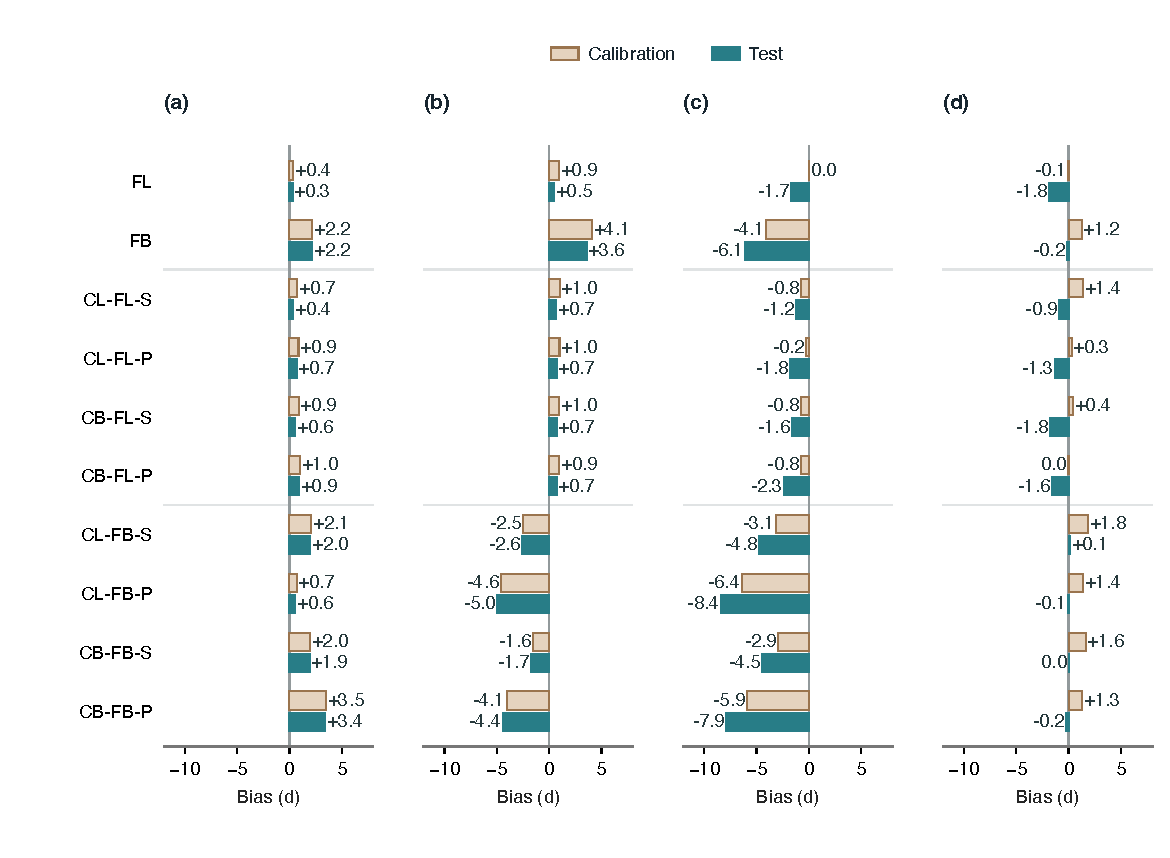
\includegraphics[width=\textwidth]{fig/paper_figures/Fig_S01.pdf}
\caption{Signed bias of process-based models (PBMs) driven by raw ERA5-Land temperature. Panels (a--d) correspond to BBCH07, BBCH65, BBCH81 and BBCH89. Light brown bars denote apparent calibration performance and blue bars denote held-out test performance. Numbers give mean signed error in days, rounded to one decimal place; negative values indicate early predictions. All bars originate at zero. Errors are averaged within sites and then equally across sites. The fixed 4 November scoring convention applies to BBCH81 and BBCH89. Values are descriptive point estimates without confidence intervals.}
\label{fig:raw_pmb_bias}
\end{figure}

\clearpage
\section{Stage-specific observation coverage and environmental-zone support}

The primary test population contains stage-specific observations at 466 sites for BBCH07, 452 for BBCH65, 346 for BBCH81 and 155 for BBCH89 (Fig.~\ref{fig:stage_observation_coverage}). Environmental-zone support and CB-FL-S error estimates are given in Table~\ref{tab:cb_fl_s_zone_support}. Observation availability is distinct from prediction attainment: sites without an observed stage date have no error estimate for that stage, even when an administrative prediction date is available.
\begin{table}[!htbp]
\centering
\caption{CB-FL-S test support and MAE by environmental zone under raw forcing. Observation and site entries give finite-scored/eligible counts; groups count those contributing finite errors. Intervals are pointwise 95\% group-bootstrap limits. A dash indicates absent observations or fewer than ten contributing groups.}
\label{tab:cb_fl_s_zone_support}
\small
\begin{tabular}{@{}lcrrrl@{}}
\toprule
Zone & BBCH & Observations & Sites & Groups & MAE (95\% interval), d \\
\midrule
EZ01 & 07 & 0/0 & 0/0 & 0 & --- \\
EZ01 & 65 & 142/145 & 5/6 & 5 & 67.14 (---) \\
EZ01 & 81 & 0/0 & 0/0 & 0 & --- \\
EZ01 & 89 & 0/0 & 0/0 & 0 & --- \\
\addlinespace
EZ02 & 07 & 282/282 & 41/41 & 36 & 13.73 (10.91--17.04) \\
EZ02 & 65 & 306/306 & 42/42 & 38 & 13.78 (11.39--16.44) \\
EZ02 & 81 & 89/89 & 12/12 & 8 & 15.10 (---) \\
EZ02 & 89 & 4/4 & 1/1 & 1 & 27.50 (---) \\
\addlinespace
EZ03 & 07 & 3865/3865 & 225/225 & 122 & 8.89 (8.23--9.58) \\
EZ03 & 65 & 4078/4078 & 198/198 & 102 & 9.01 (7.93--10.28) \\
EZ03 & 81 & 2564/2564 & 111/111 & 51 & 17.39 (14.97--20.23) \\
EZ03 & 89 & 113/113 & 6/6 & 4 & 21.59 (---) \\
\addlinespace
EZ04 & 07 & 700/700 & 104/104 & 66 & 8.39 (7.31--9.70) \\
EZ04 & 65 & 712/712 & 109/109 & 62 & 8.46 (7.41--9.72) \\
EZ04 & 81 & 487/487 & 95/95 & 56 & 11.87 (9.58--14.48) \\
EZ04 & 89 & 249/249 & 68/68 & 37 & 10.40 (8.40--12.84) \\
\addlinespace
EZ05 & 07 & 221/226 & 94/96 & 62 & 9.42 (7.92--10.96) \\
EZ05 & 65 & 223/228 & 95/97 & 62 & 9.54 (8.16--11.00) \\
EZ05 & 81 & 614/614 & 128/128 & 74 & 10.45 (8.47--13.38) \\
EZ05 & 89 & 484/484 & 80/80 & 46 & 13.64 (11.24--16.13) \\
\bottomrule
\end{tabular}
\end{table}


\clearpage
\begin{figure}[!htbp]
\centering
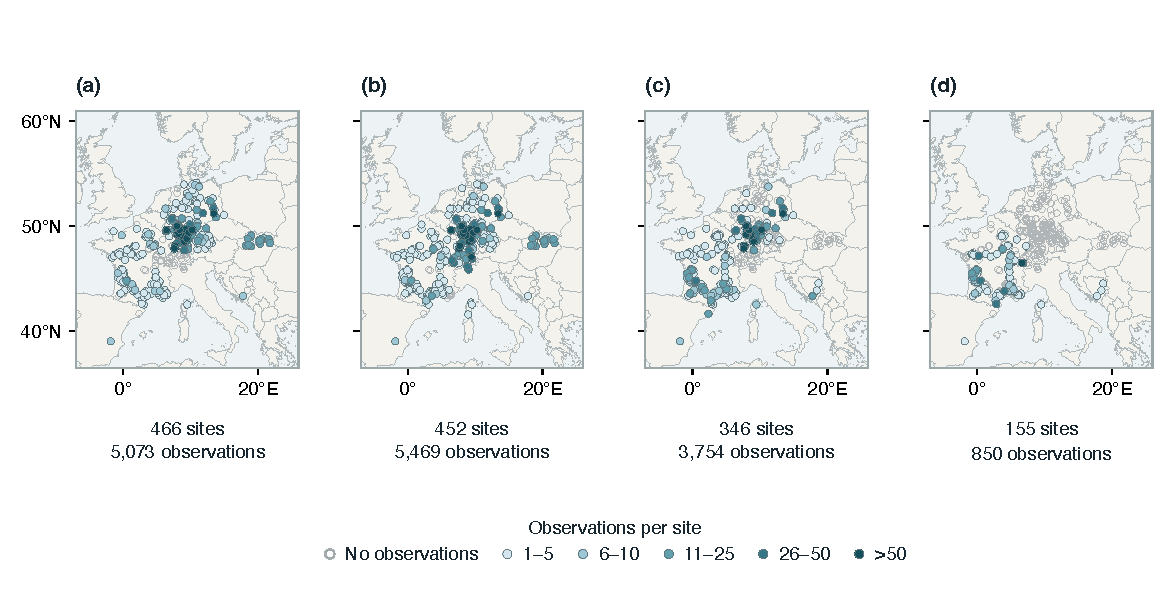
\includegraphics[width=\textwidth]{fig/paper_figures/Fig_S02.pdf}
\caption{Stage-specific observation availability in the primary test partition. Panels (a--d) show BBCH07, 65, 81 and 89, respectively, in the same stage order as the main performance figure. All 635 source-qualified test sites are represented in each panel. Filled circles indicate sites with accepted observations of that stage; colour denotes the number of observation records per site, and pale open circles indicate no observations of that stage. Counts below each panel give sites with observations and their total records. Repeated accepted observations remain separate, and counts are independent of model prediction availability. Coincident locations can overlap; no spatial interpolation or coordinate jitter is applied. The fixed 4 November scoring rule supplies dates for late or unattained BBCH81/89 predictions but does not supply missing observations.}
\label{fig:stage_observation_coverage}
\end{figure}

\clearpage
\section{Paired DEM analysis and regional terrain semivariograms}

The DEM comparison uses the locked process predictions from all ten structures. An observation contributes when its scoring date is finite in both temperature arms of every structure. This common population contains 5,066 BBCH07, 5,435 BBCH65, 3,754 BBCH81 and 850 BBCH89 observations at 633 sites in 355 original independence groups. It excludes seven budburst and 34 flowering observations; no BBCH81 or BBCH89 observation is lost. The primary analysis retains the 4 November scoring convention. Model-specific finite-pair results are retained separately as a sensitivity to the common-cohort requirement.

For observation $i$, the fixed-model loss is $\overline{L}_{i,t}=10^{-1}\sum_{m=1}^{10}|e_{i,m,t}|$, where $t$ denotes RAW or DEM forcing. The paired benefit is $\overline{L}_{i,\mathrm{RAW}}-\overline{L}_{i,\mathrm{DEM}}$. Benefits are averaged over observations within each site and stage, then equally over contributing sites. Overall estimates average the four stage means without renormalizing missing stages. Squared and signed errors are averaged separately; RMSE is the square root of the corresponding mean squared error. A site counts as improved when its fixed-model mean MAE is strictly smaller under DEM forcing. Stage-specific benefits across terrain classes are shown in Fig.~\ref{fig:dem_terrain_stages}. Alternative structures are fixed comparisons, not independent replicates or an ensemble of predicted dates.

Uncertainty uses 2,000 bootstrap samples of original independence groups with replacement, preserving all sites and stages within each sampled group. Within each draw, sites retain equal weight multiplied by their group's draw multiplicity. Pointwise 95\% percentile intervals require at least ten contributing groups per stage and at least 95\% finite draws. Differences between high and low terrain classes use the same group draws in both classes; they are not inferred from overlap between separate intervals. All terrain and regional associations are exploratory, without adjustment for multiple comparisons.

Terrain heterogeneity motivates spatially differentiated weather-data requirements \citep{zhaoDemand2015}. The regional semivariogram diagnostic here has a separately specified spatial support and does not reproduce that study's implementation. Verified, georeferenced GLO-30 overview extracts, originally cached for relief rendering, supply average-resampled elevations at approximately 300--500~m resolution. They are distinct from the native DEM pixels used for site terrain derivatives and from ERA5-Land model orography. Each original weather cell is represented by a 20$\times$20-km square centred on its grid coordinate, sampled at 500-m spacing in a local azimuthal equidistant projection. Nearest overview pixels supply sampled elevations, and the country-boundary land mask excludes sea. At least 90\% of the 1,600 lattice positions must contain valid land elevations.

The isotropic empirical semivariogram is
\begin{equation}
\widehat\gamma(h)=\frac{1}{2N_h}\sum_{(i,j)\in B_h}(z_i-z_j)^2,
\end{equation}
where $B_h$ contains pairs in a 0.5-km distance bin and $N_h$ is its pair count. Actual mean pair distances represent bins through a maximum lag of 10~km; each retained bin requires at least 100 pairs. A spherical model is fitted by pair-count-weighted least squares:
\begin{equation}
\gamma(h)=\begin{cases}C\{1.5(h/a)-0.5(h/a)^3\},&0<h<a,\\C,&h\geq a,\end{cases}
\end{equation}
where $C$ is the sill in m$^2$ and $a$ is the range in km. The nugget is fixed at zero for this smoothed-elevation diagnostic; it is not estimated as a separate measurement-error component. Sill is bounded between zero and ten times sampled elevation variance, and range between 0.5 and 30~km. Four initial ranges (2, 5, 10 and 20~km) are evaluated, retaining the fit with the smallest weighted residual sum of squares.

A supported sill requires at least 16 empirical lag bins, successful optimization, an unweighted fit $R^2\geq0.7$, an inactive upper sill bound and a range no greater than 8~km. The range criterion places the estimated plateau inside the observed lag support. Unsupported values are missing rather than replaced by local variance or an extrapolated sill. Of 1,791 cells, 475 meet these criteria, 1,262 lack a supported plateau and 54 have insufficient land coverage. Supported sills occur at 644 calibration sites and 149 test sites; the latter contribute 148 sites to the common prediction cohort. Sill tertiles are calculated from supported calibration sites only. Smoothed input, isotropy, the zero-nugget assumption, land coverage and the finite window limit this regional diagnostic; the sill sample is not representative of all test sites.

\begin{figure}[!htbp]
\centering
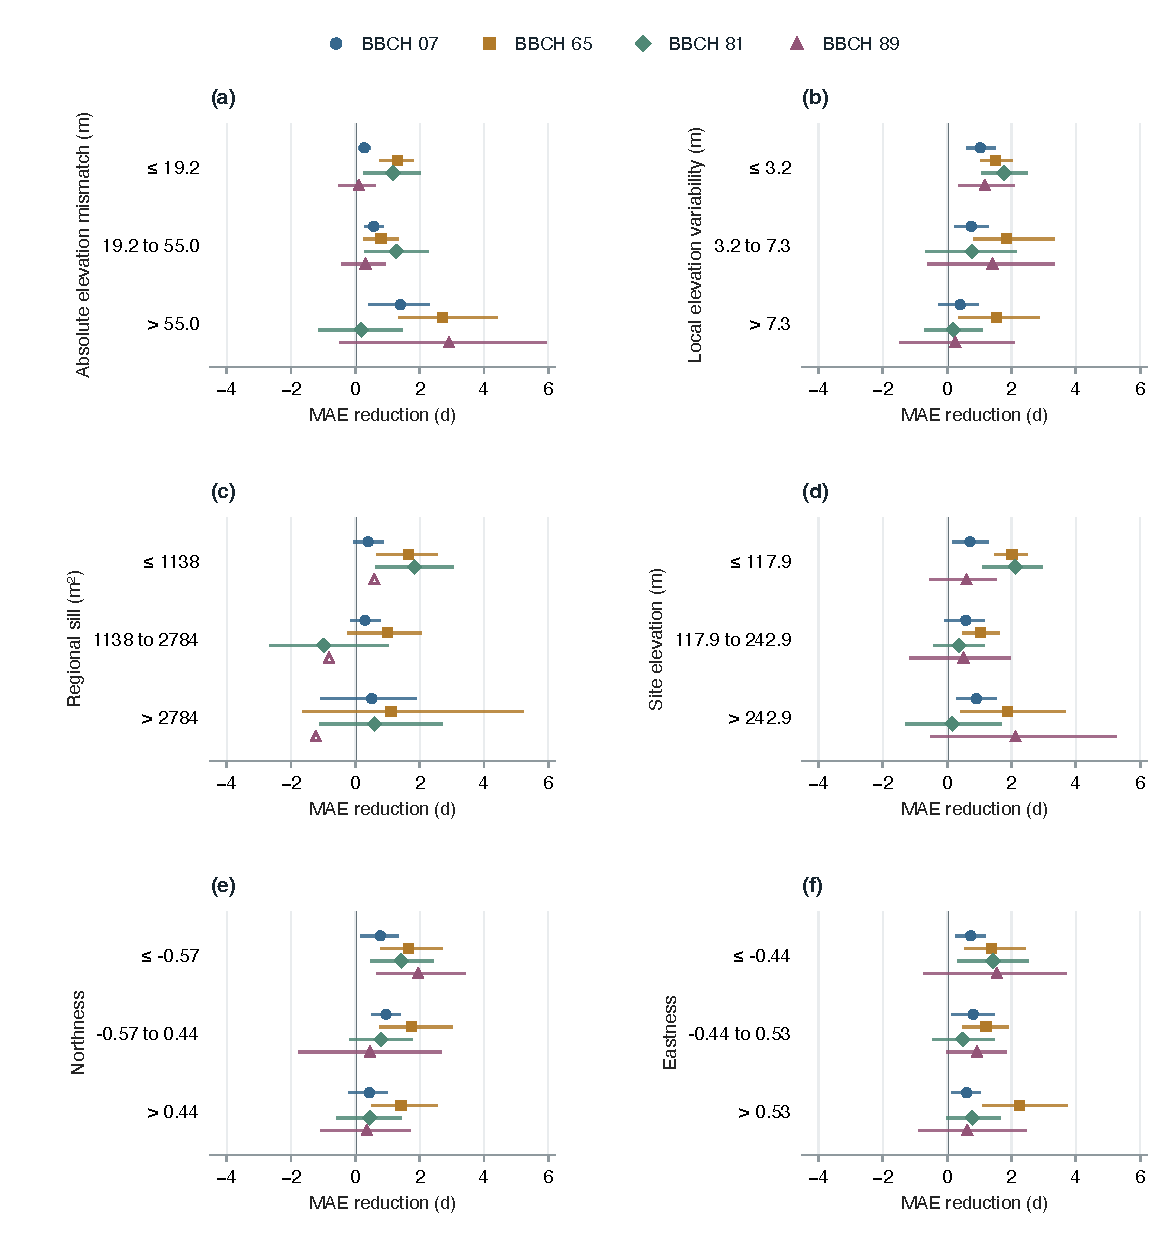
\includegraphics[width=\textwidth]{fig/paper_figures/Fig_S03.pdf}
\caption{Stage-specific DEM benefits across calibration-defined terrain classes: (a) absolute elevation mismatch, (b) local elevation variability, (c) supported regional semivariogram sill, (d) site elevation, (e) northness and (f) eastness. Points are equal-site MAE reductions averaged across the ten fixed PBMs; positive values indicate improvement. Horizontal intervals are pointwise 95\% original-group bootstrap intervals. Open symbols identify insufficient group support. Northness and eastness are the cosine and sine of aspect; their dimensionless values run from $-1$ to $+1$. Class boundaries are rounded for display. Missing terrain and unsupported sill fits retain separate records in the analytical tables. All panels share the same horizontal scale.}
\label{fig:dem_terrain_stages}
\end{figure}

\clearpage
\section{Additional DEM metrics and regional support}

Signed bias and RMSE respond differently to elevation correction (Fig.~\ref{fig:dem_bias_rmse}). Across equally weighted stages, RMSE decreased from 16.80 to 15.61~d. Maturity/harvest MAE decreased even as its mean bias became more negative; signed errors alone therefore do not determine predictive accuracy. Regional contrasts retain stage-specific support (Table~\ref{tab:dem_zone_effects}). Missing stages cannot contribute an error estimate, and sparse regional samples do not acquire confidence intervals through averaging alternative models.

\begin{figure}[!htbp]
\centering
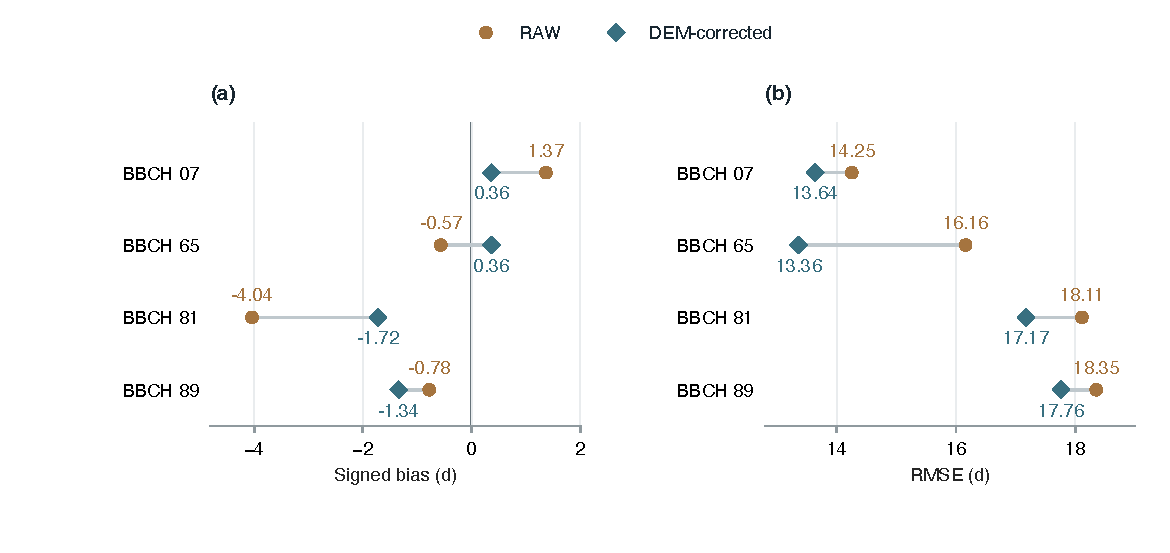
\includegraphics[width=\textwidth]{fig/paper_figures/Fig_S04.pdf}
\caption{Changes in (a) signed bias and (b) RMSE after DEM correction, averaged at the appropriate error scale across the ten fixed PBMs. RAW and DEM values use identical observations, sites and stage weights. Text gives values in days; points are estimates without confidence intervals, and connecting lines pair the temperature treatments. The 4 November scoring convention remains in force for BBCH81 and BBCH89.}
\label{fig:dem_bias_rmse}
\end{figure}
\clearpage
\begin{longtable}{@{}lcrrr@{}}
\caption{Paired DEM effects by environmental zone. MAE reduction is the mean across ten fixed PMBs, with sites and stages weighted as described in the main text. Intervals are pointwise 95\% original-group bootstrap intervals; a dash denotes insufficient support. Counts refer to the common twenty-arm cohort.}\label{tab:dem_zone_effects}\\
\toprule
Zone & BBCH & Sites/groups & MAE reduction, d & 95\% interval, d \\
\midrule\endfirsthead
\toprule Zone & BBCH & Sites/groups & MAE reduction, d & 95\% interval, d \\ \midrule\endhead
EZ01 & 07 & 0/0 & --- & --- \\
EZ01 & 65 & 5/5 & 45.26 & --- \\
EZ01 & 81 & 0/0 & --- & --- \\
EZ01 & 89 & 0/0 & --- & --- \\
\addlinespace
EZ02 & 07 & 41/36 & 1.74 & -0.04 to 3.40 \\
EZ02 & 65 & 42/38 & 1.47 & -0.37 to 3.33 \\
EZ02 & 81 & 12/8 & -1.79 & --- \\
EZ02 & 89 & 1/1 & 22.17 & --- \\
\addlinespace
EZ03 & 07 & 225/122 & 0.84 & 0.44 to 1.26 \\
EZ03 & 65 & 198/102 & -0.08 & -0.50 to 0.36 \\
EZ03 & 81 & 111/51 & 0.98 & -0.14 to 2.16 \\
EZ03 & 89 & 6/4 & 5.22 & --- \\
\addlinespace
EZ04 & 07 & 104/66 & 0.28 & -0.54 to 0.93 \\
EZ04 & 65 & 109/62 & 1.41 & 0.78 to 1.99 \\
EZ04 & 81 & 95/56 & -0.59 & -1.48 to 0.45 \\
EZ04 & 89 & 68/37 & 1.28 & -0.26 to 2.75 \\
\addlinespace
EZ05 & 07 & 93/61 & 0.51 & -0.10 to 1.06 \\
EZ05 & 65 & 93/60 & 3.16 & 2.75 to 3.56 \\
EZ05 & 81 & 128/74 & 2.22 & 1.31 to 2.99 \\
EZ05 & 89 & 80/46 & 0.13 & -0.73 to 0.73 \\
\addlinespace
\bottomrule
\end{longtable}


\clearpage
\section{Residual-learning bias diagnostics}

Main-text Figs.~9 and 10 use common finite-scoring populations across all ten structures. The ML contrast requires both RAW process and RAW hybrid scores; the DEM contrast within hybrids requires RAW and DEM hybrid scores. Both retain the same 15,105 observations at 633 sites in 355 original independence groups: 5,066 BBCH07, 5,435 BBCH65, 3,754 BBCH81 and 850 BBCH89 observations. The corresponding site counts are 463, 447, 346 and 155. Seven budburst and 34 flowering observations lack common finite support; BBCH81/89 scoring assignments remain unchanged.

For aggregate summaries, absolute errors are averaged across the ten fixed models at each observation, then within sites and equally across sites. This averages losses rather than predicted dates. Overall gains average the four stage-specific means. Pointwise 95\% percentile intervals use 2,000 draws of original independence groups, with at least ten groups per stage and 95\% finite draws required. Missing stages are not renormalized into an overall estimate. Environmental-zone summaries retain the original zone assignments and describe subsets of the primary held-out population. A site is improved when its average MAE across the ten hybrids decreases under DEM forcing; unchanged sites remain in the denominator.

The decrease in DEM benefit after residual learning is the paired contrast $\{MAE_{\mathrm{P,RAW}}-MAE_{\mathrm{P,DEM}}\}-\{MAE_{\mathrm{H,RAW}}-MAE_{\mathrm{H,DEM}}\}$, where P denotes process-only predictions and H denotes hybrids. Positive values indicate a smaller DEM benefit for hybrids. The process and hybrid comparisons contain identical observations, verified by observation identity, and retain the same model, site and stage weights. Each bootstrap draw applies the same original-group multiplicities to both DEM benefits; percentile limits are calculated from their within-draw difference. This is a contrast between separately fitted prediction workflows, not a causal effect of residual learning on temperature accuracy. Relative DEM gains divide each workflow's absolute gain by its own RAW MAE.

Signed-bias diagnostics retain the original model-specific scoring populations, separately for RAW and DEM temperature and calibration and testing. These populations can differ slightly from the common cohorts used in main-text Figs.~9 and 10.

Absolute stage-specific bias moved closer to zero after residual learning in 55 of the 80 held-out model--temperature--stage comparisons (Fig.~\ref{fig:ml_bias_supplement}). Hybrid signed bias ranged from $-2.69$ to $+0.71$~d. A smaller mean signed error does not necessarily imply smaller individual prediction errors; signed bias and MAE quantify distinct aspects of predictive performance. Calibration values are apparent performance after training on calibration-only out-of-fold residuals.

\begin{figure}[!htbp]
\centering
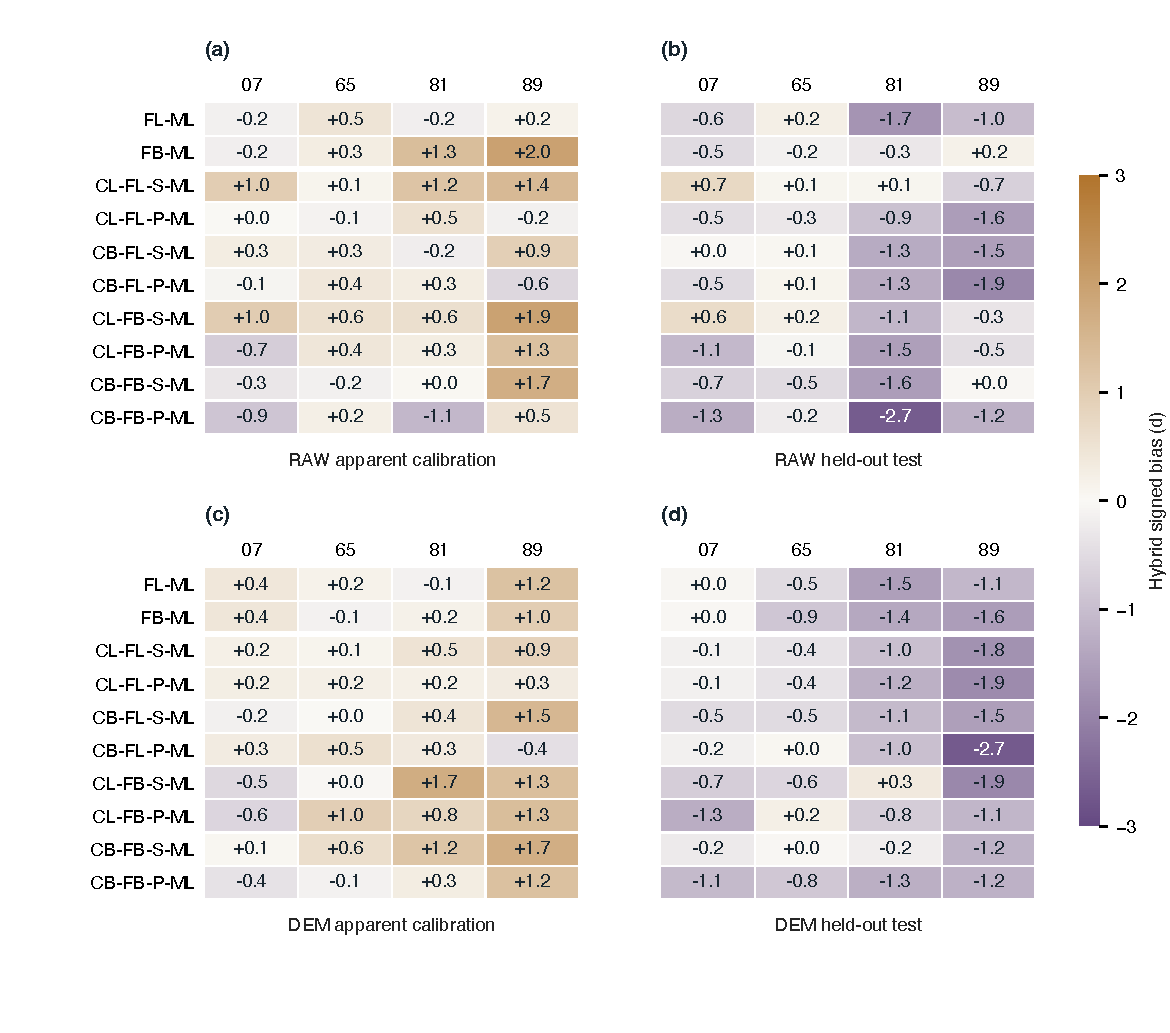
\includegraphics[width=\textwidth]{fig/paper_figures/Fig_S05.pdf}
\caption{Signed bias of residual-learning hybrids. Panels (a,b) show RAW apparent calibration and held-out test performance; panels (c,d) show the corresponding DEM results. Columns give BBCH07, 65, 81 and 89; model order matches main-text Fig.~9. Signed bias is predicted minus observed date, averaged within sites and then equally across sites. Negative values indicate earlier predictions and positive values later predictions. All panels share a zero-centred colour scale; numbers are descriptive point estimates in days, rounded to one decimal place. Calibration scores are apparent. BBCH81/89 retain the fixed 4 November scoring convention.}
\label{fig:ml_bias_supplement}
\end{figure}

\clearpage
\begingroup
\small
\setstretch{1.0}
\bibliographystyle{plainnat}
\bibliography{references/Phenological}
\endgroup
\end{document}
